\newpage

\chapter{Sprint 5: Reporting and Analytics Dashboard}

\cfoot{\thepage}

\parindent=0.5in
\onehalfspacing

\section{Introduction}

Sprint 5, titled "Reporting and Analytics Dashboard," implements comprehensive reporting and analytics capabilities enabling data-driven decision making through intelligent visualization, flexible filtering, and multi-format export functionality. This sprint addresses user stories US-012 (Analytics Dashboard), US-013 (Custom Reports), and US-014 (Data Export) from Chapter 2's product backlog.

Network operations generate massive data volumes across sites, equipment, maintenance activities, incidents, and alerts established in Sprints 1-4. The reporting system aggregates this data presenting unified views of network health, operational efficiency, and service quality metrics supporting the stakeholder requirements identified in Chapter 2.

Advanced visualization techniques including interactive charts, trend analysis, and comparative statistics enable stakeholders to identify patterns, detect anomalies, and make informed decisions. The implementation leverages data from all previous sprints providing comprehensive operational intelligence.

\section{Sprint Backlog}

During sprint planning, we defined the tasks required for Sprint 5 implementation. Table 7.1 presents the sprint backlog with user stories, tasks, complexity assessments, and effort estimates.

\begin{table}[H]
\centering
\small
\begin{tabular}{|p{2.5cm}|p{4cm}|p{3.2cm}|p{2.2cm}|p{1.5cm}|}
\hline
\textbf{Functionality} & \textbf{User Story} & \textbf{Tasks} & \textbf{Complexity} & \textbf{Estimate} \\
\hline

\multirow{3}{2.5cm}{Analytics Dashboard (US-012)} & 
\multirow{3}{4cm}{As manager, I want comprehensive analytics dashboard for operations overview}
& Create dashboard layout & Medium & 3h \\
\cline{3-5}
& & Aggregate statistics & Hard & 3h \\
\cline{3-5}
& & Implement KPIs & Medium & 2h \\
\hline

\multirow{3}{2.5cm}{Interactive Charts} & 
\multirow{3}{4cm}{As engineer, I want interactive charts for data visualization}
& Implement chart components & Medium & 3h \\
\cline{3-5}
& & Add filtering capability & Medium & 2h \\
\cline{3-5}
& & Enable drill-down & Hard & 2h \\
\hline

\multirow{3}{2.5cm}{Custom Reports (US-013)} & 
\multirow{3}{4cm}{As manager, I want to generate custom reports with date ranges}
& Create report builder & Medium & 3h \\
\cline{3-5}
& & Implement date filters & Easy & 2h \\
\cline{3-5}
& & Add preset options & Easy & 1h \\
\hline

\multirow{3}{2.5cm}{Breakdown Analysis} & 
\multirow{3}{4cm}{As engineer, I want detailed breakdown analysis with metrics}
& Calculate MTTR/MTBF & Hard & 3h \\
\cline{3-5}
& & Show impact analysis & Medium & 2h \\
\cline{3-5}
& & Create analysis view & Easy & 1h \\
\hline

\multirow{3}{2.5cm}{Export CSV (US-014)} & 
\multirow{3}{4cm}{As manager, I want to export reports to CSV format}
& Implement CSV generation & Medium & 2h \\
\cline{3-5}
& & Handle large datasets & Medium & 2h \\
\cline{3-5}
& & Optimize encoding & Easy & 1h \\
\hline

\multirow{3}{2.5cm}{Export PDF (US-014)} & 
\multirow{3}{4cm}{As admin, I want to export reports to PDF format}
& Implement PDF with jsPDF & Hard & 3h \\
\cline{3-5}
& & Add progress tracking & Medium & 2h \\
\cline{3-5}
& & Format multi-page layout & Medium & 2h \\
\hline

\multirow{3}{2.5cm}{Performance KPIs} & 
\multirow{3}{4cm}{As manager, I want to view key performance indicators}
& Calculate uptime metrics & Medium & 2h \\
\cline{3-5}
& & Calculate response time & Medium & 2h \\
\cline{3-5}
& & Calculate efficiency metrics & Easy & 1h \\
\hline

\multirow{3}{2.5cm}{Date Range Filter} & 
\multirow{3}{4cm}{As user, I want to filter reports by date period}
& Implement date picker & Easy & 2h \\
\cline{3-5}
& & Add preset shortcuts & Easy & 2h \\
\cline{3-5}
& & Add custom range & Medium & 2h \\
\hline

\end{tabular}
\caption{Sprint 5 Backlog with Task Breakdown}
\label{tab:sprint5_backlog}
\end{table}

The backlog totals 50 hours across eight major functionalities. PDF generation complexity stems from client-side rendering requirements and memory management. Data aggregation requires efficient query optimization processing thousands of historical records from Sprints 2-4.

\section{Conceptual Design}

This section presents the conceptual design models guiding Sprint 5 implementation.

\subsection{Class Diagram}

Figure 7.1 presents the class diagram illustrating the reporting system architecture integrating data from all previous sprints.

\begin{figure}[H]
    \centering
    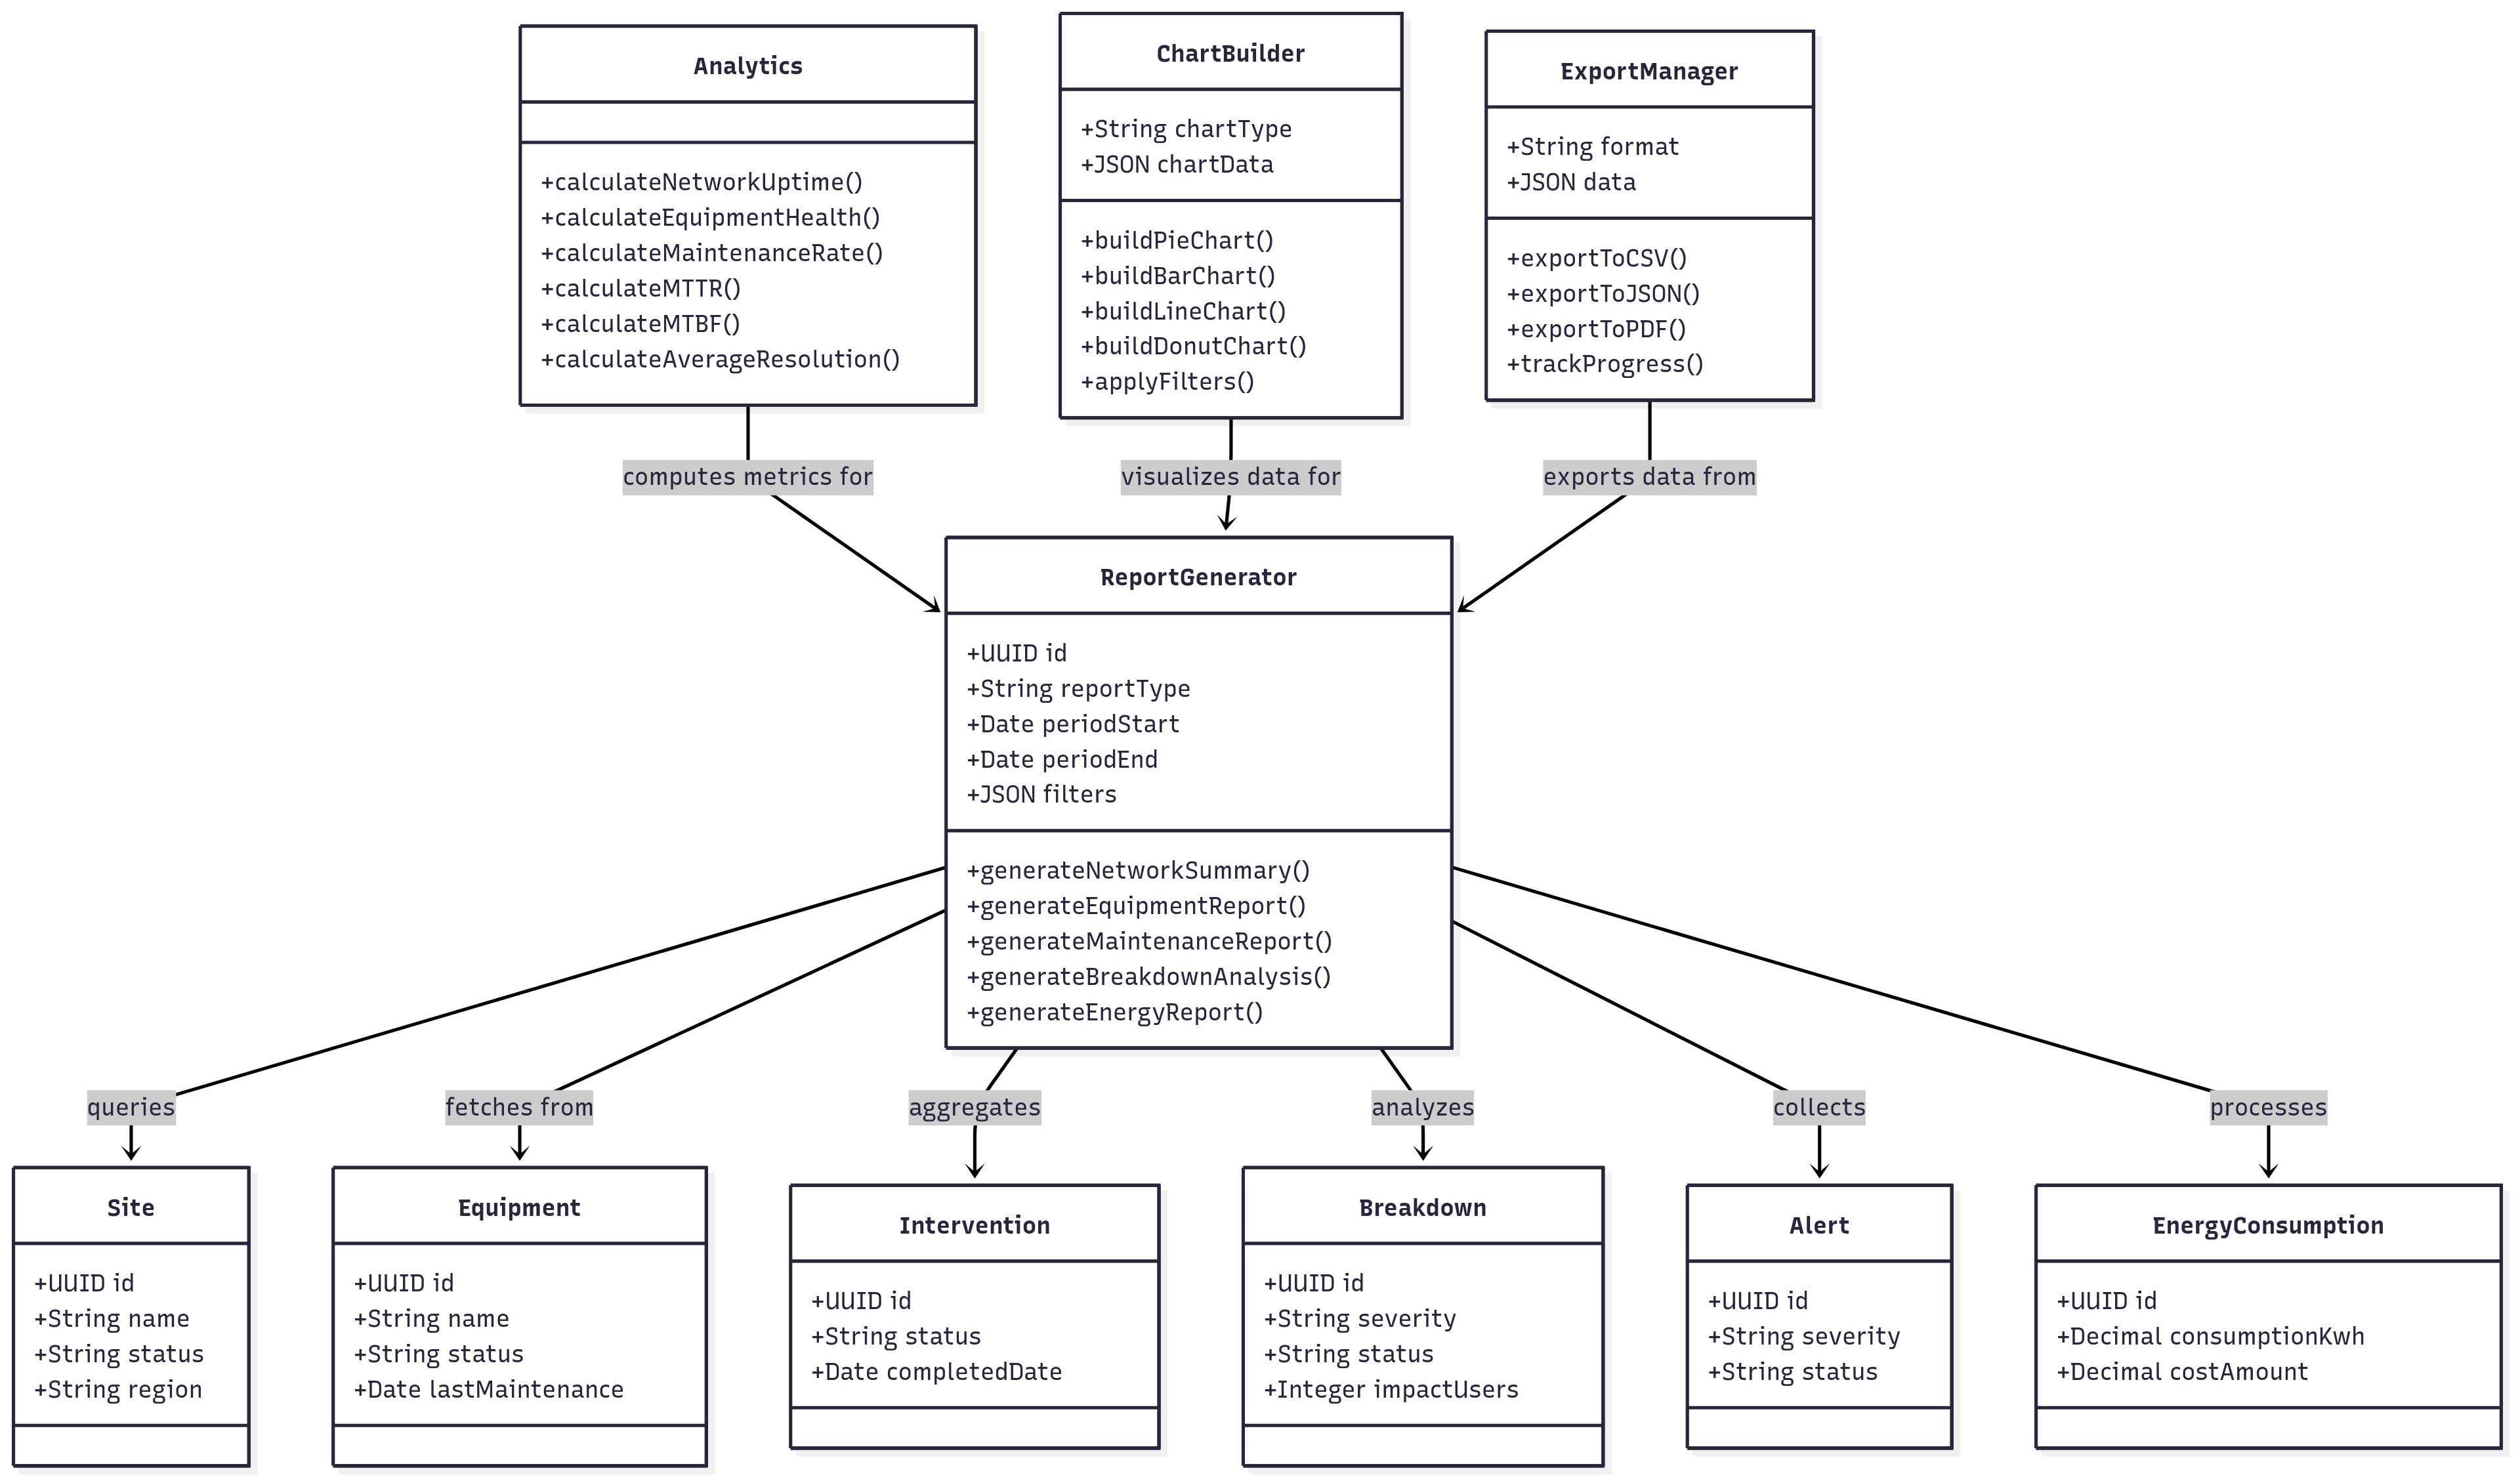
\includegraphics[width=0.95\linewidth]{img/chap_07/sprint5_class_diagram.png}
    \caption{Class Diagram - Reporting and Analytics System}
    \label{fig:class_diagram_sprint5}
\end{figure}

The class diagram (Figure 7.1) illustrates the reporting architecture aggregating data from Site, Equipment, Intervention, Breakdown, Alert, and EnergyConsumption entities established in previous sprints.

The ReportGenerator class creates various report types including network summary aggregating site and equipment data from Sprint 1 and 2, equipment status reports, maintenance history from Sprint 3, and breakdown analysis. The class supports flexible date range selection, customizable filtering, and multiple output formats.

The Analytics class calculates key performance indicators including network uptime percentage, Mean Time To Repair (MTTR) from breakdown data, Mean Time Between Failures (MTBF) from equipment history, and response time metrics from intervention tracking. These calculations leverage the comprehensive operational data collected throughout all sprints.

The ChartBuilder transforms aggregated data into visualization formats supporting line charts for trends, bar charts for comparisons, pie charts for distributions, and area charts for cumulative metrics. The ExportManager handles data export in CSV, JSON, and PDF formats with proper encoding and formatting.

\subsection{Use Case Diagram}

Figure 7.2 presents the use case diagram showing role-based permissions for reporting functionality, following the inheritance hierarchy established in Chapter 3.

\begin{figure}[H]
    \centering
    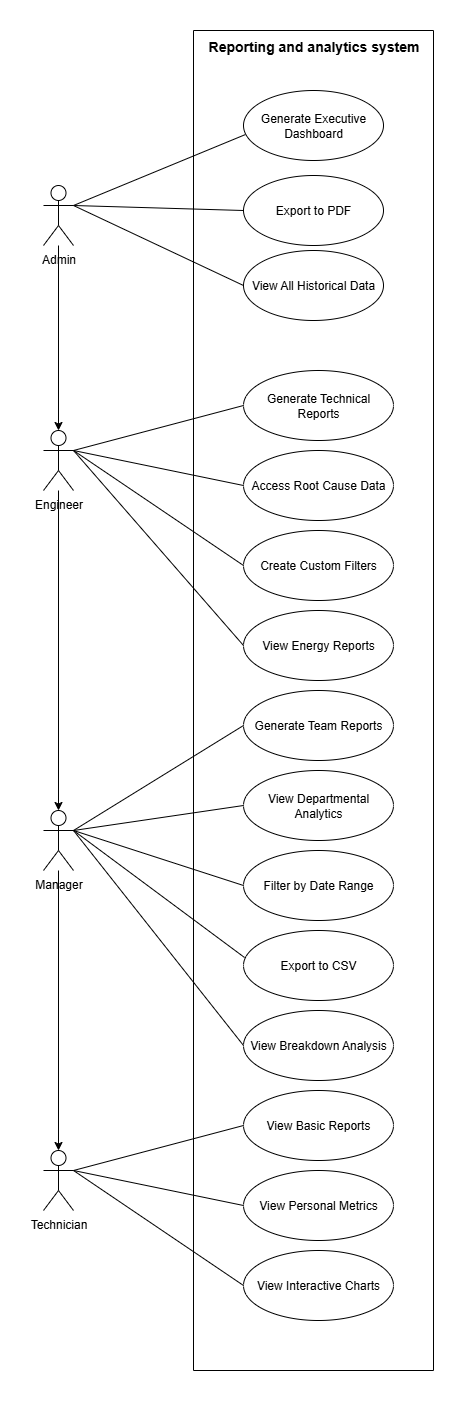
\includegraphics[width=0.45\linewidth]{img/chap_07/sprint5_usecase_diagram.png}
    \caption{Use Case Diagram - Sprint 5 with Role Inheritance}
    \label{fig:use_case_diagram_sprint5}
\end{figure}

The use case diagram (Figure 7.2) demonstrates the established role inheritance hierarchy. Field Technicians access basic reports showing personal performance metrics and assigned tasks. Managers inherit all technician capabilities while adding team reports, departmental analytics, and CSV export for data sharing. Network Engineers inherit all manager capabilities while adding technical reports, root cause analysis capabilities, and custom filtering for detailed investigation. Administrators inherit all engineer capabilities while possessing executive dashboards, PDF export for formal reporting, and report scheduling capabilities.

\textbf{Use Case Description: Generate Report}

Table 7.2 provides detailed information on the "Generate Report" use case as representative of Sprint 5 reporting functionality.

\begin{table}[H]
\centering
\small
\begin{tabular}{|p{3cm}|p{8.5cm}|}
\hline
\textbf{Element} & \textbf{Description} \\
\hline
\textbf{Use Case Name} & Generate Report \\
\hline
\textbf{Primary Actors} & Network Engineer, Operations Manager, Administrator \\
\hline
\textbf{Description} & Generate comprehensive reports aggregating operational data across selected time periods with customizable filtering \\
\hline
\textbf{Pre-condition} & User authenticated with appropriate role; Historical data available from Sprints 1-4; Aggregation services operational \\
\hline
\textbf{Post-condition} & Report generated and displayed; Export options available; Activity logged for audit \\
\hline
\textbf{Main Scenario} & 
1. User navigates to reports dashboard
2. User selects report type (network, equipment, maintenance, breakdown)
3. User sets date range using presets or custom selection
4. User applies optional filters (site, severity, status)
5. User clicks "Generate Report" button
6. System validates parameters
7. System aggregates data from multiple tables
8. System calculates performance metrics
9. System generates visualizations
10. System displays complete report
11. System enables export options
\\
\hline
\textbf{Alternative Flows} & 
A1 - PDF Export: User selects "Export PDF", system shows progress tracking through five stages, generates PDF with proper formatting, triggers download when complete
A2 - Preset Selection: User selects quick preset (Last 7 Days, Last 30 Days), system auto-fills date range
\\
\hline
\textbf{Exception Scenarios} & 
E1: Insufficient data for selected period → Display warning with alternative suggestions
E2: Large dataset exceeds memory → Initiate background processing with email notification
E3: Export failure → Log error details and offer retry options
\\
\hline
\end{tabular}
\caption{Detailed Use Case Description - Generate Report}
\label{tab:generate_report_usecase}
\end{table}

\section{Sequence Diagrams}

This section presents sequence diagrams detailing the main processes implemented in Sprint 5.

\subsection{Generate Report Process}

Figure 7.3 demonstrates the complete workflow for generating analytical reports with data aggregation from multiple sources.

\begin{figure}[H]
    \centering
    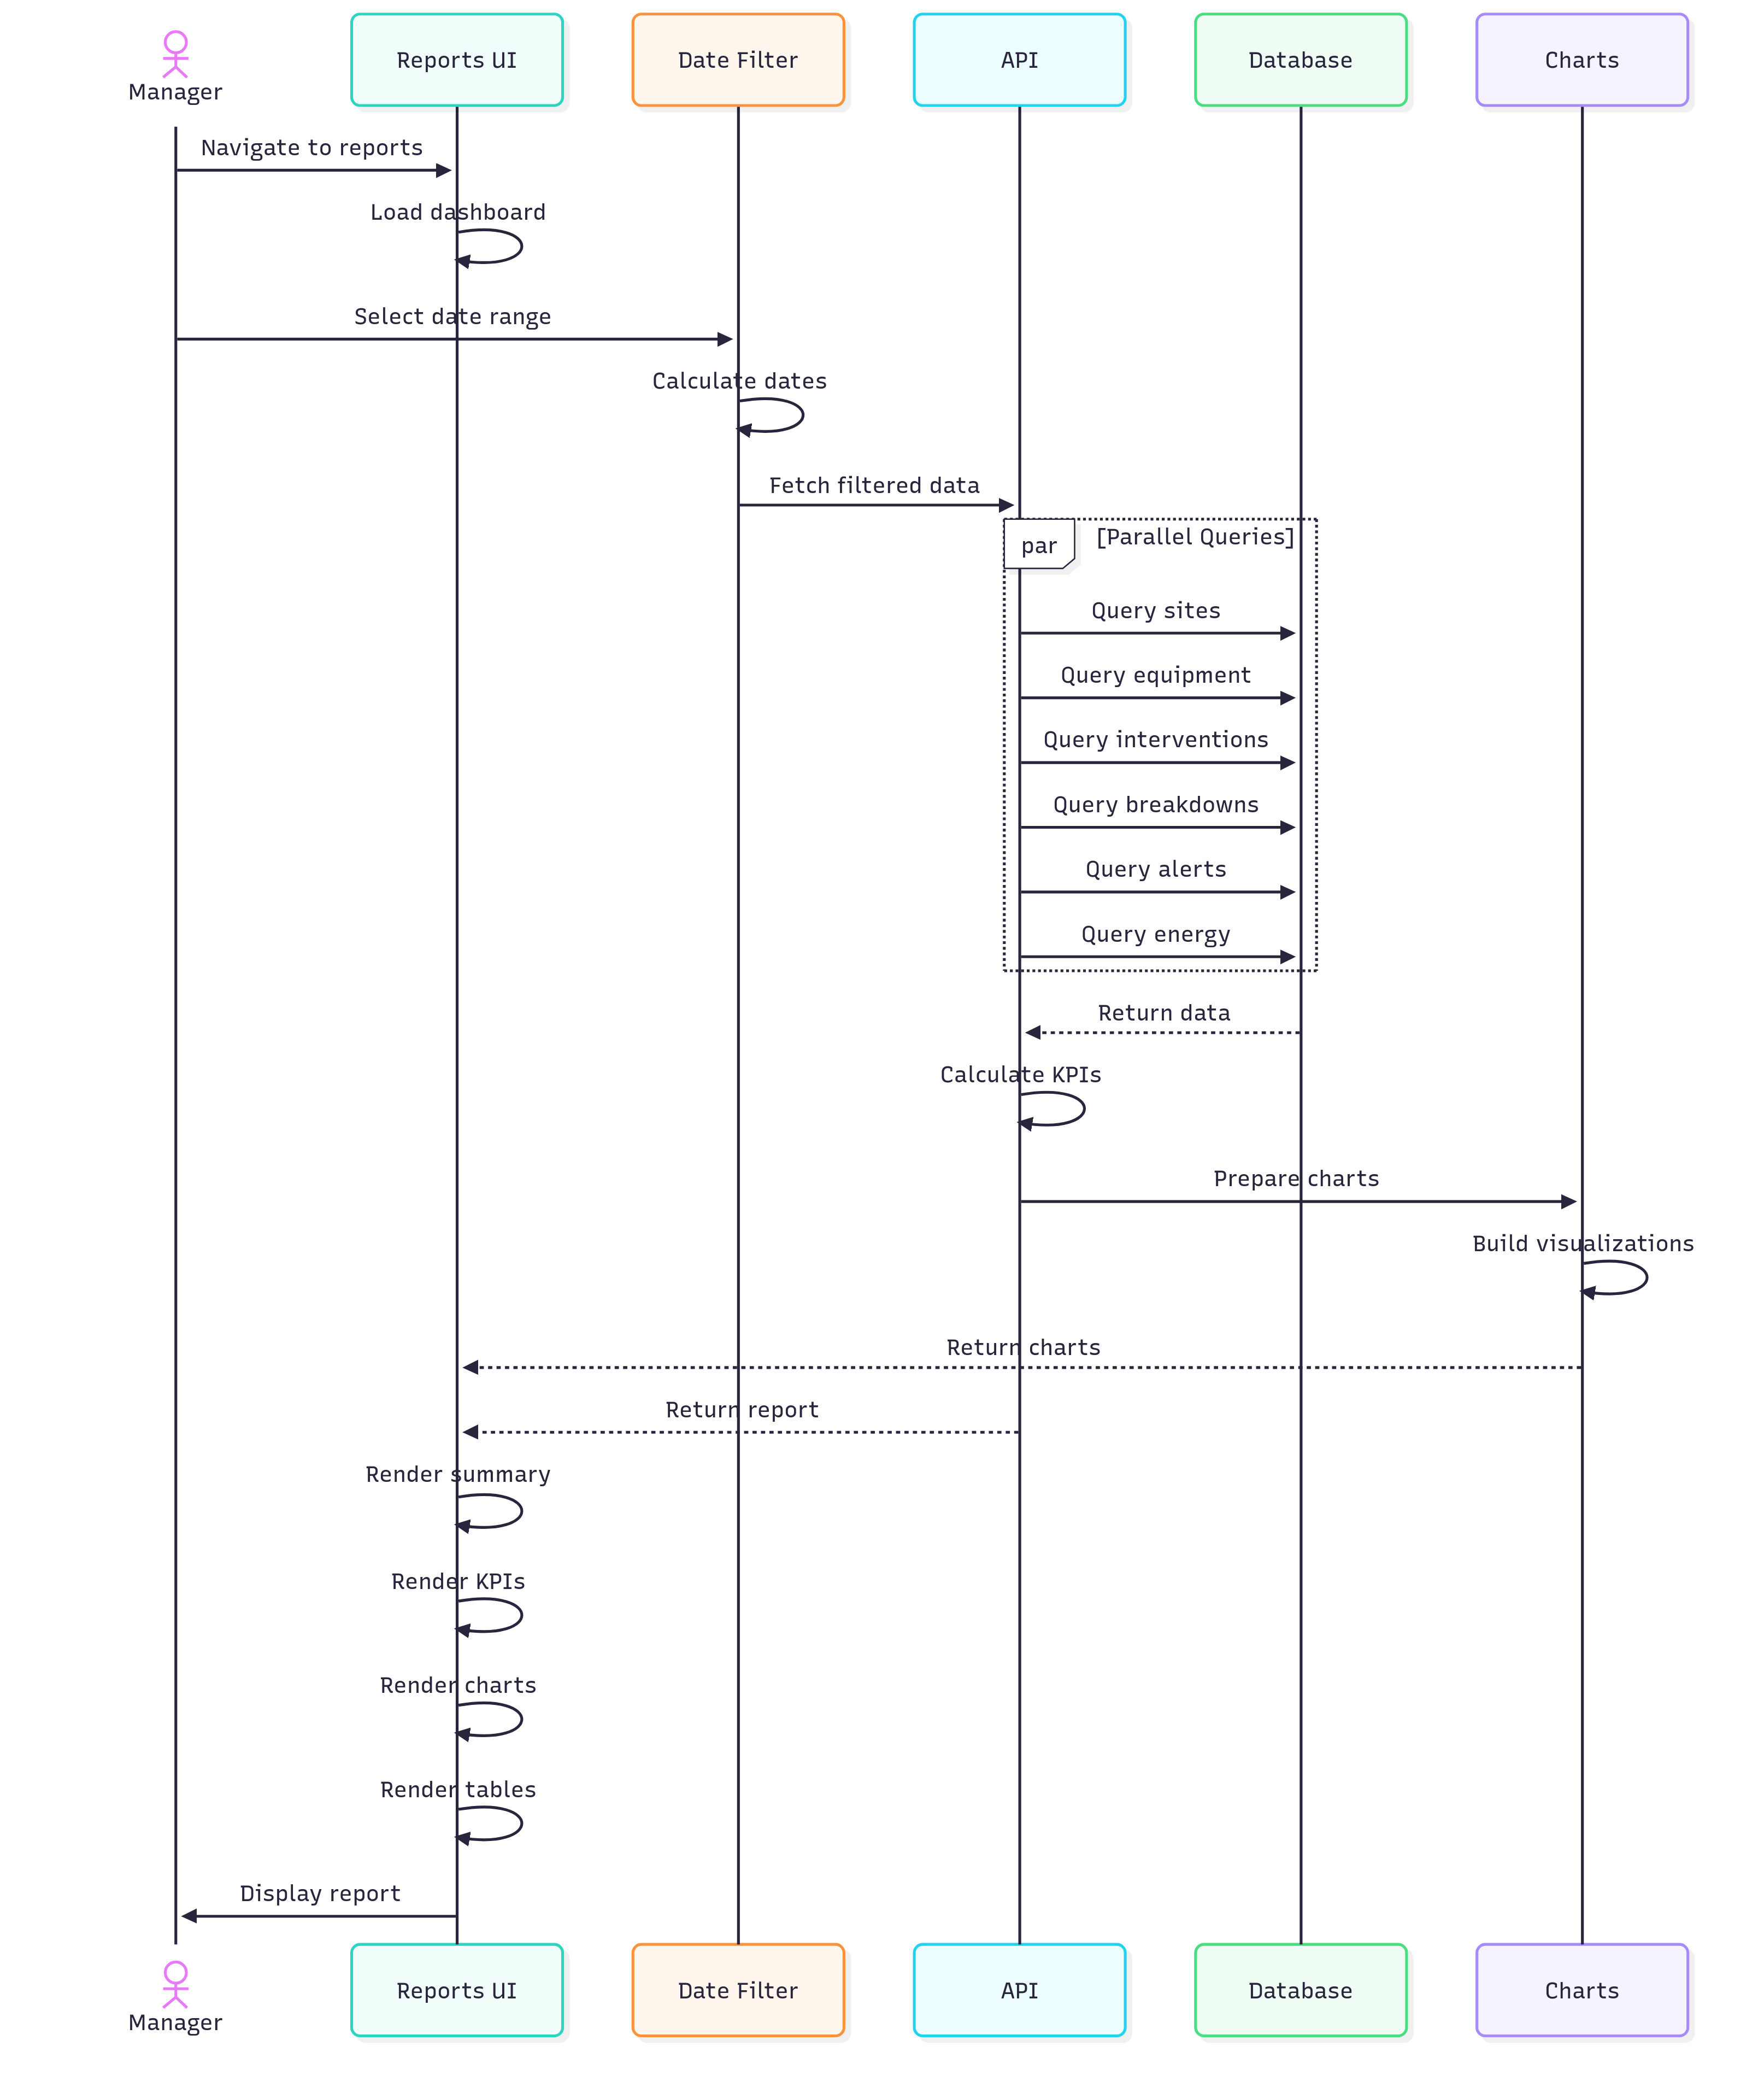
\includegraphics[width=0.95\linewidth]{img/chap_07/sprint5_sequence_report.png}
    \caption{Sequence Diagram - Generate Report Process}
    \label{fig:sequence_generate_report}
\end{figure}

\textbf{Note on Sequence Diagram:} Following UML sequence diagram standards, return messages should use dashed arrows (-->) while request messages use solid arrows (->), clearly distinguishing between calls and responses.

The generate report sequence (Figure 7.3) demonstrates the workflow for creating analytical reports. An authorized user navigates to the reports dashboard and selects desired report type (network summary, equipment status, maintenance history, or breakdown analysis). The user configures the report by setting date range using quick presets or custom selection, applying optional filters for specific sites or equipment, and selecting visualization preferences.

Upon clicking "Generate Report", the system validates parameters ensuring dates are logical and filters are compatible. The ReportGenerator component queries multiple data sources including sites table from Sprint 1, equipment records from Sprint 2, interventions and breakdowns from Sprint 3, and alerts and energy data from Sprint 4. The Analytics engine calculates key performance indicators including uptime percentage, MTTR, MTBF, and efficiency metrics. The ChartBuilder transforms aggregated data into visualization components. The complete report displays with interactive charts, summary statistics, and detailed tables.

\subsection{Export Data Process}

Figure 7.4 illustrates the workflow for exporting report data to CSV, JSON, and PDF formats.

\begin{figure}[H]
    \centering
    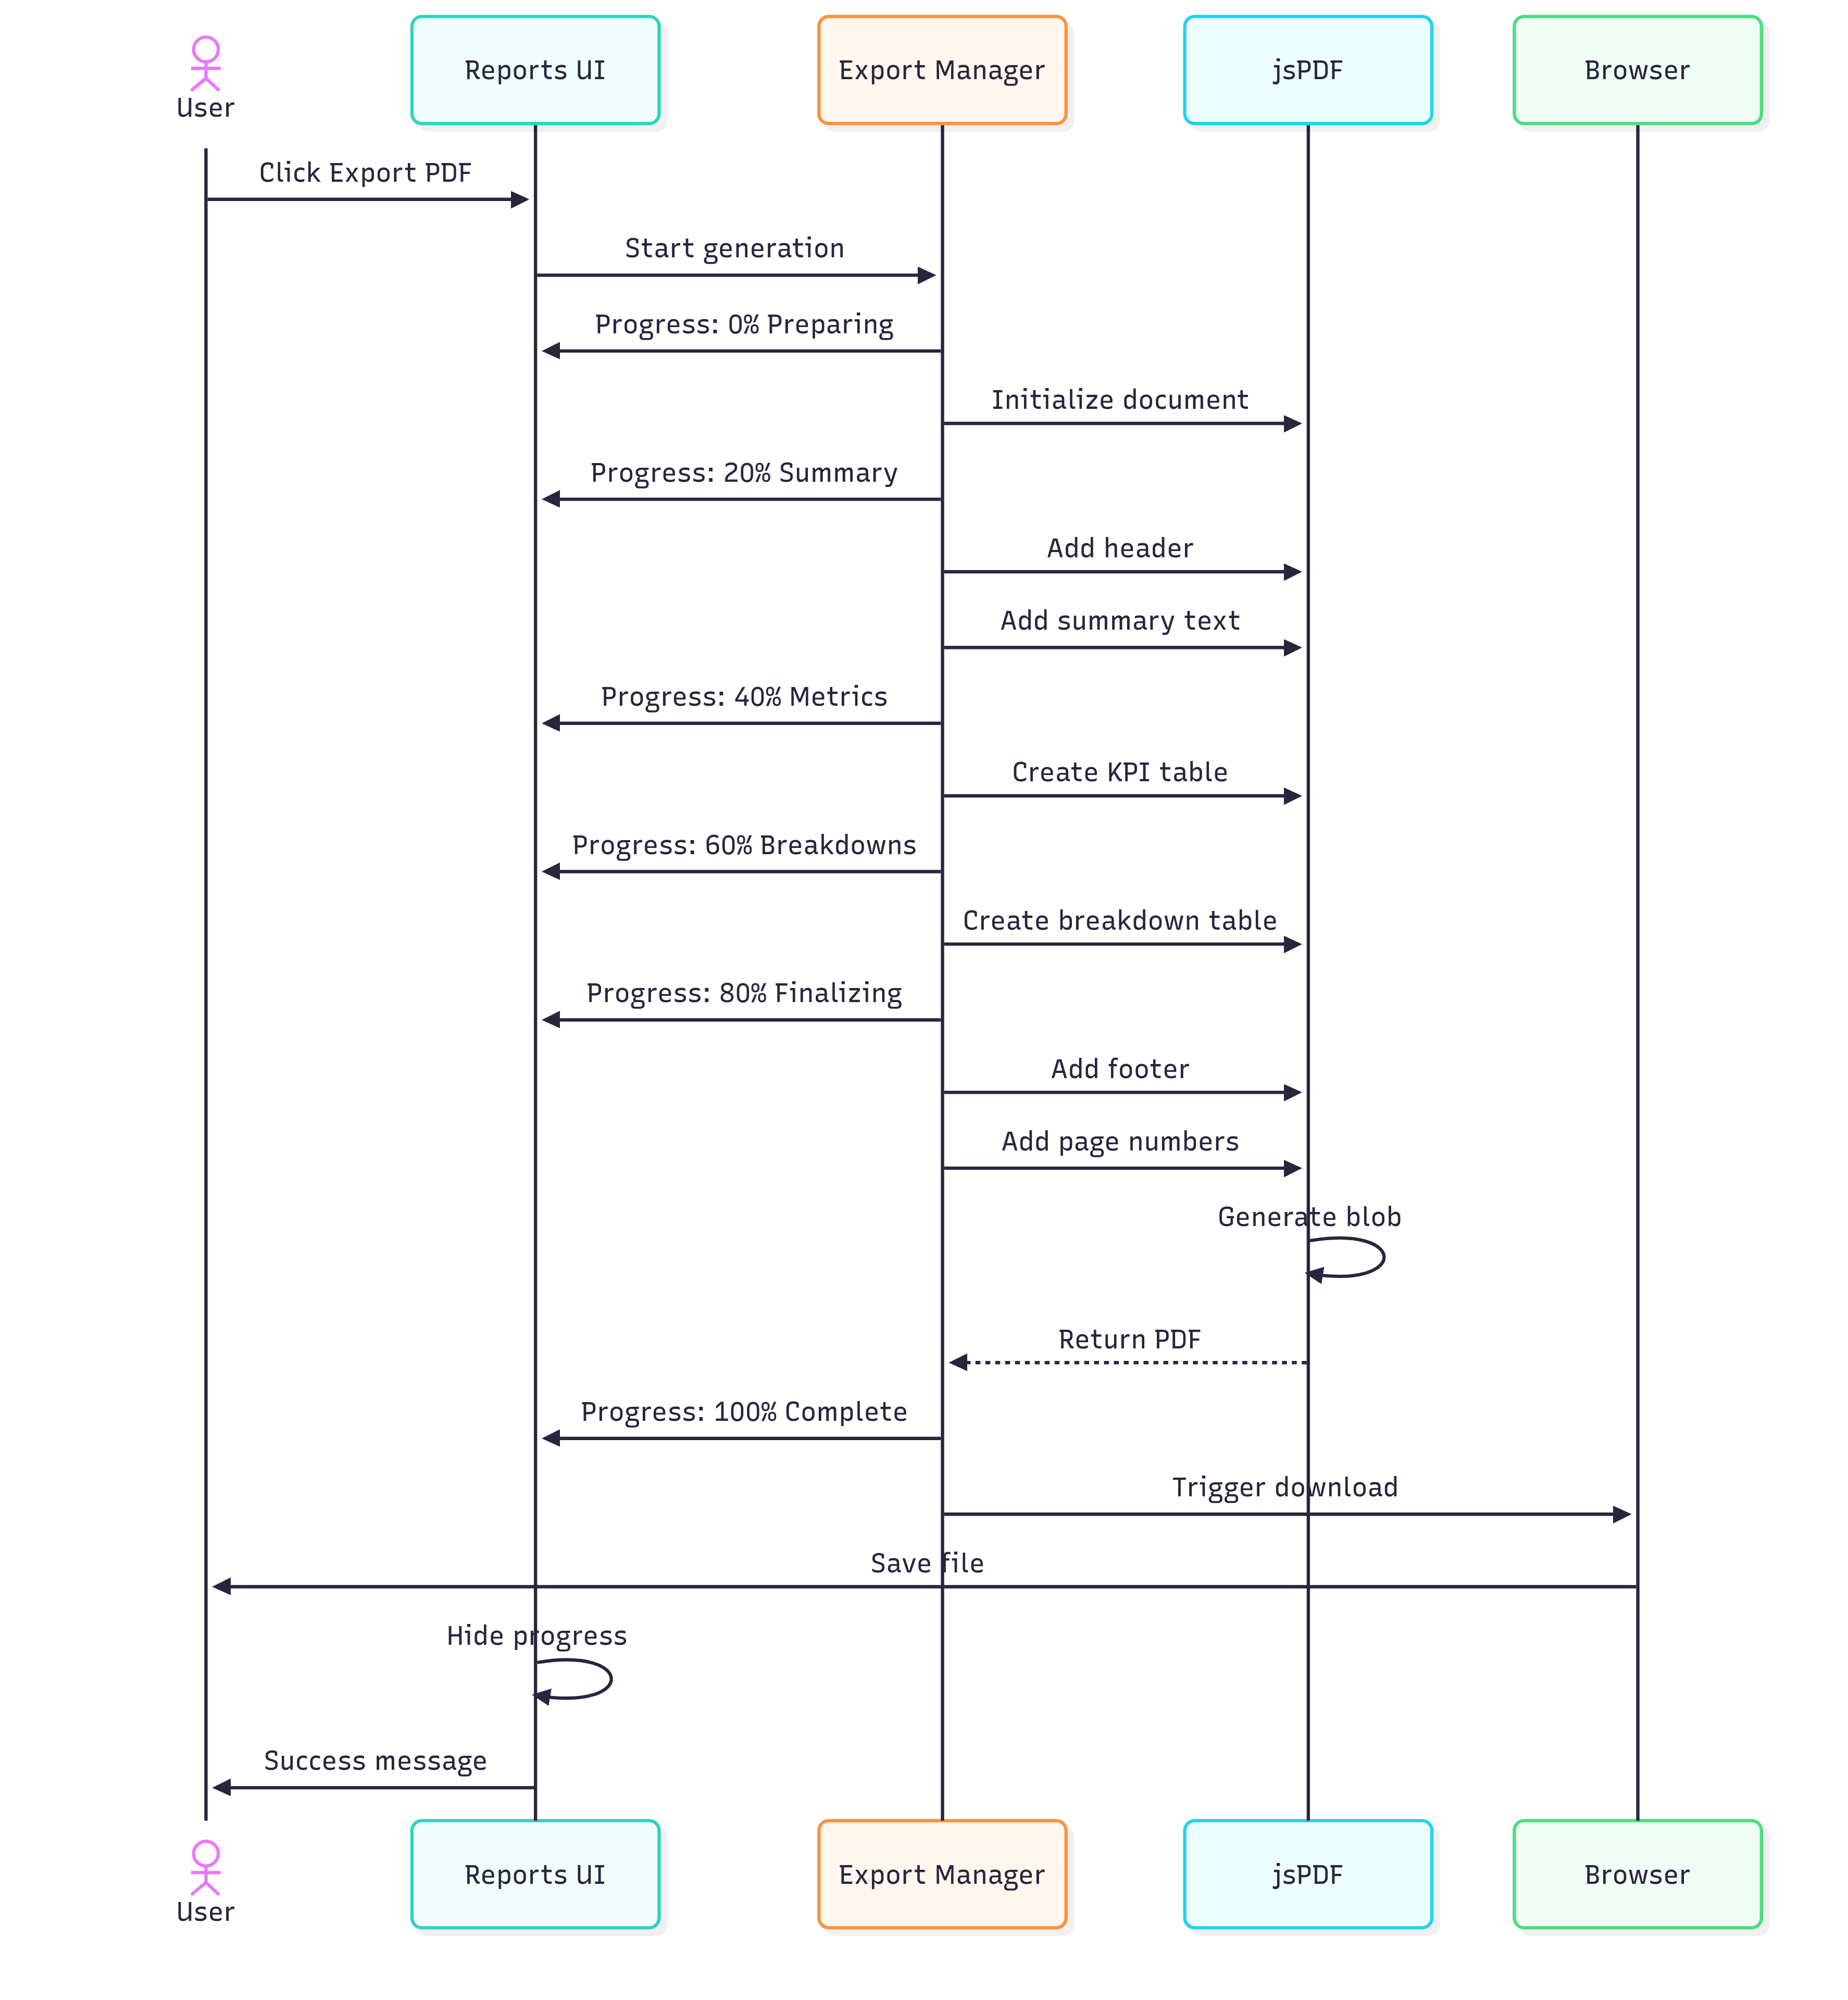
\includegraphics[width=0.95\linewidth]{img/chap_07/sprint5_sequence_export.png}
    \caption{Sequence Diagram - Export Data Process}
    \label{fig:sequence_export_data}
\end{figure}

The export data sequence (Figure 7.4) demonstrates multi-format export capabilities. When a user selects export format (CSV, JSON, or PDF), the ExportManager validates the request ensuring appropriate permissions. For CSV export, the system serializes tabular data with proper encoding and triggers immediate download. For JSON export, the system structures hierarchical data with metadata and initiates download.

For PDF export, the process is more complex due to client-side generation constraints. The system initializes jsPDF library, creates staged generation with five phases (preparation, summary, metrics, breakdowns, finalization), updates progress bar showing 0-100% completion, formats multi-page layout with headers and footers, and triggers download when complete. Progress tracking provides user feedback during generation preventing perceived freezing.

\section{Implementation}

This section presents screenshots illustrating the interfaces developed during Sprint 5 implementation.

\subsection{Analytics Dashboard Overview}

Figure 7.5 illustrates the main analytics dashboard providing comprehensive operational overview.

\begin{figure}[H]
    \centering
    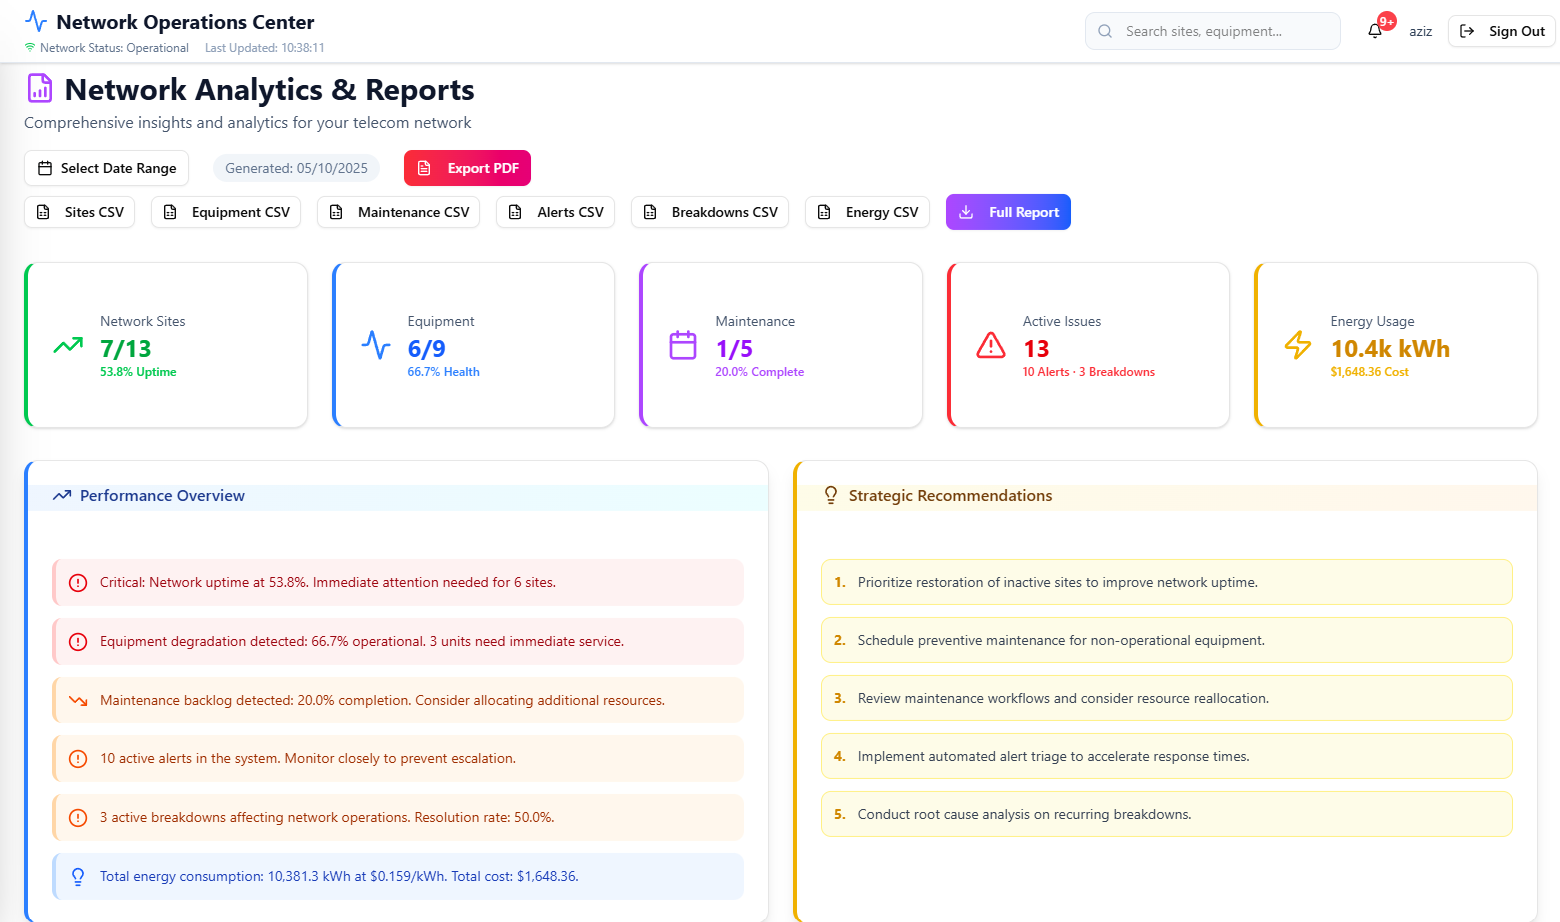
\includegraphics[width=0.9\linewidth]{img/chap_07/screenshot_analytics_dashboard.png}
    \caption{Analytics Dashboard with KPIs and Intelligent Insights}
    \label{fig:analytics_dashboard}
\end{figure}

The analytics dashboard (Figure 7.5) displays critical metrics including network uptime percentage calculated from site availability data, equipment health index aggregating operational status, maintenance completion rate from intervention tracking, and breakdown resolution efficiency from incident management. The intelligent summary section provides narrative insights with color-coded status indicators highlighting areas requiring attention. Quick insight cards show total sites count, online percentage, equipment total, and active alerts providing at-a-glance operational status.

\subsection{Interactive Charts Visualization}

Figure 7.6 displays interactive charts enabling data exploration and trend analysis.

\begin{figure}[H]
    \centering
    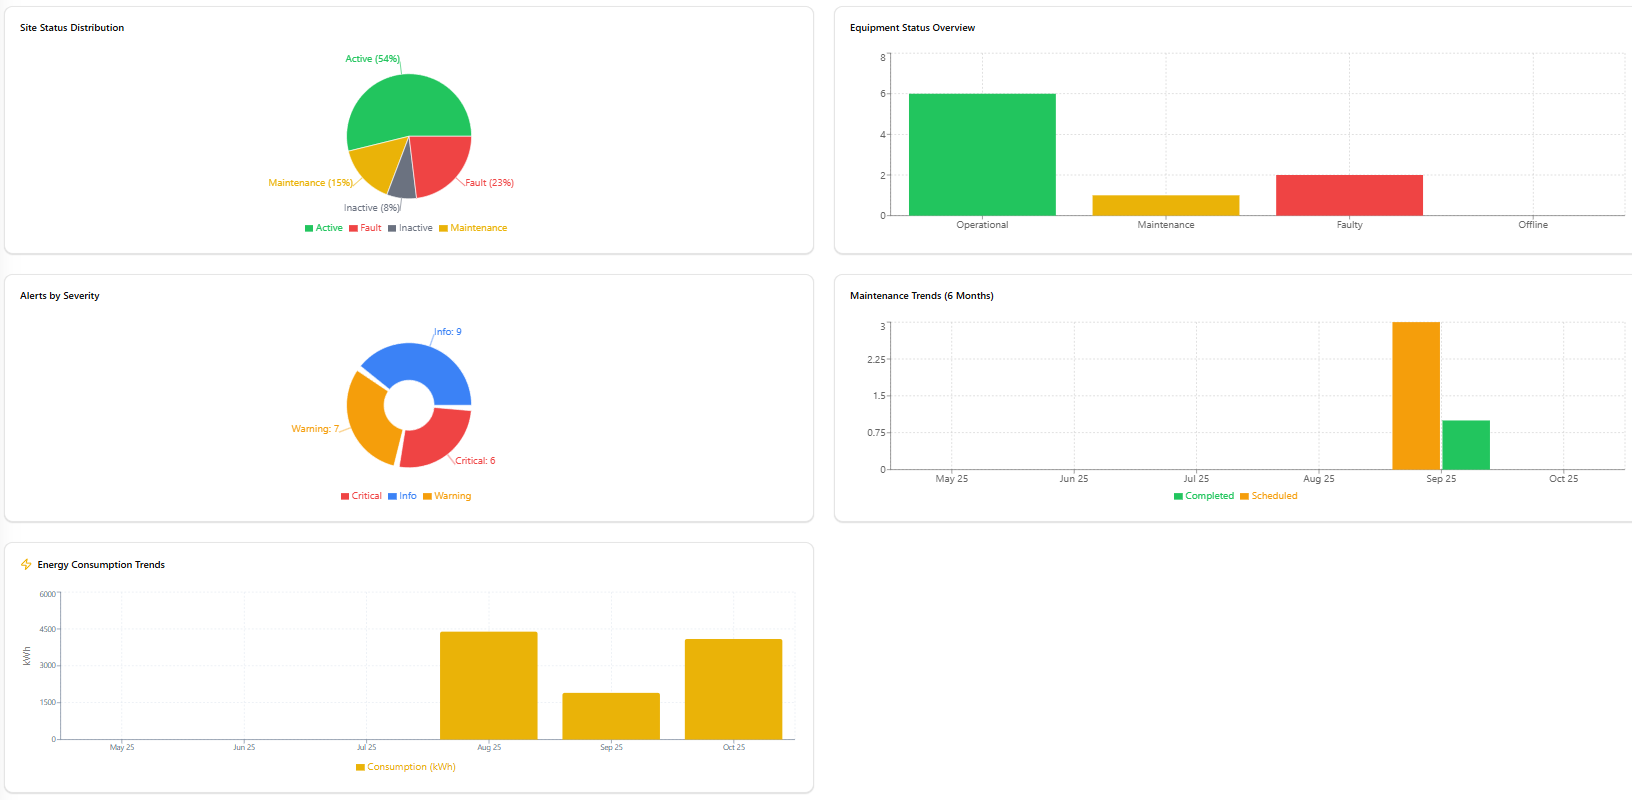
\includegraphics[width=0.9\linewidth]{img/chap_07/screenshot_charts_visualization.png}
    \caption{Interactive Charts Showing Operational Trends}
    \label{fig:charts_visualization}
\end{figure}

The charting system (Figure 7.6) uses Recharts library providing pie charts for status distribution showing breakdown by category, bar charts for comparative analysis across sites or time periods, and line charts for trend visualization tracking metrics over time. Interactive features enable data filtering by clicking legend items, drill-down capability accessing underlying data, hover tooltips displaying exact values, and responsive design ensuring accessibility across desktop and mobile devices.

\subsection{Breakdown Analysis Report}

Figure 7.7 presents detailed breakdown analysis with performance metrics.

\begin{figure}[H]
    \centering
    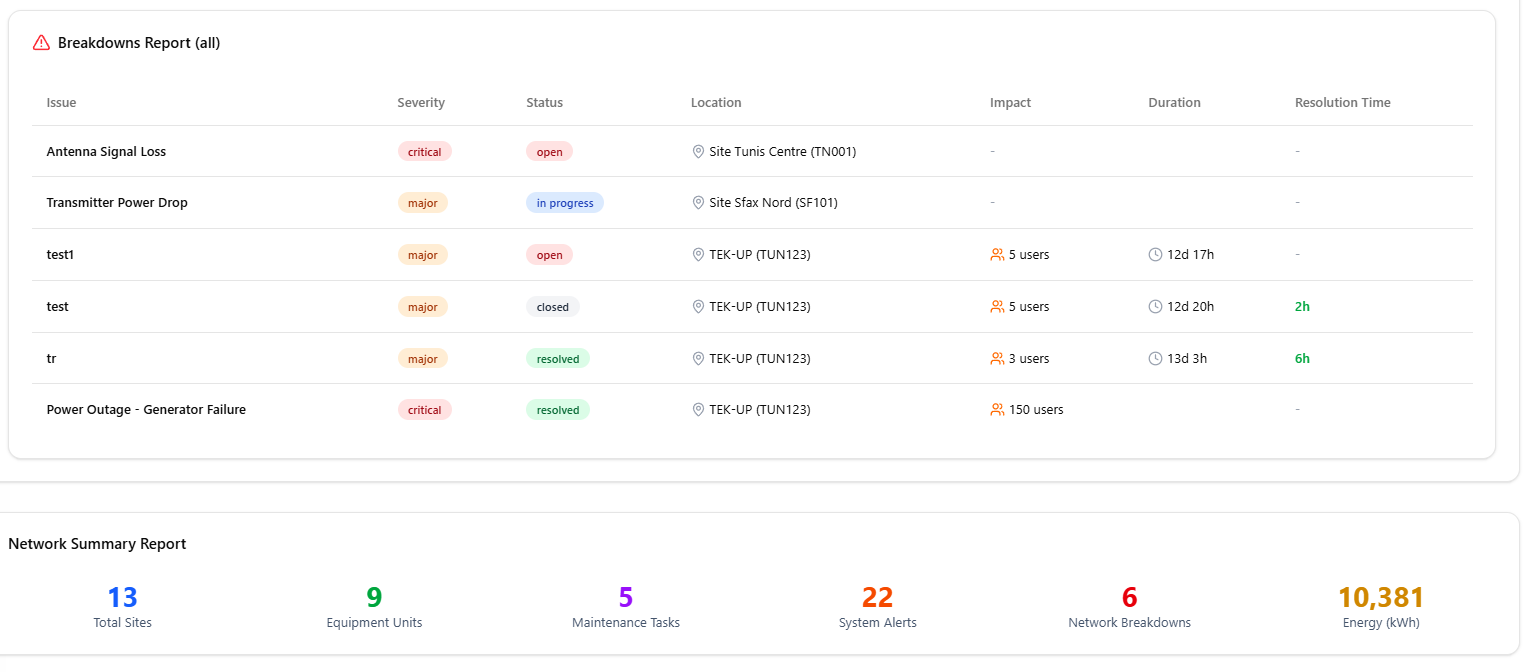
\includegraphics[width=0.9\linewidth]{img/chap_07/screenshot_breakdown_analysis.png}
    \caption{Breakdown Analysis with Performance Metrics}
    \label{fig:breakdown_analysis}
\end{figure}

The breakdown analysis interface (Figure 7.7) displays comprehensive statistics including total breakdowns over selected period, active issues requiring attention, critical count needing immediate response, resolution status showing workflow progress, and impact statistics quantifying affected users. The detailed table presents breakdown descriptions, severity classifications with color coding, current status in resolution workflow, affected site locations, estimated user impact, and resolution times enabling MTTR calculation. Color-coded badges enable quick priority identification supporting efficient incident management.

\subsection{Date Range Filter Interface}

Figure 7.8 illustrates the date range filter with quick presets and custom selection.

\begin{figure}[H]
    \centering
    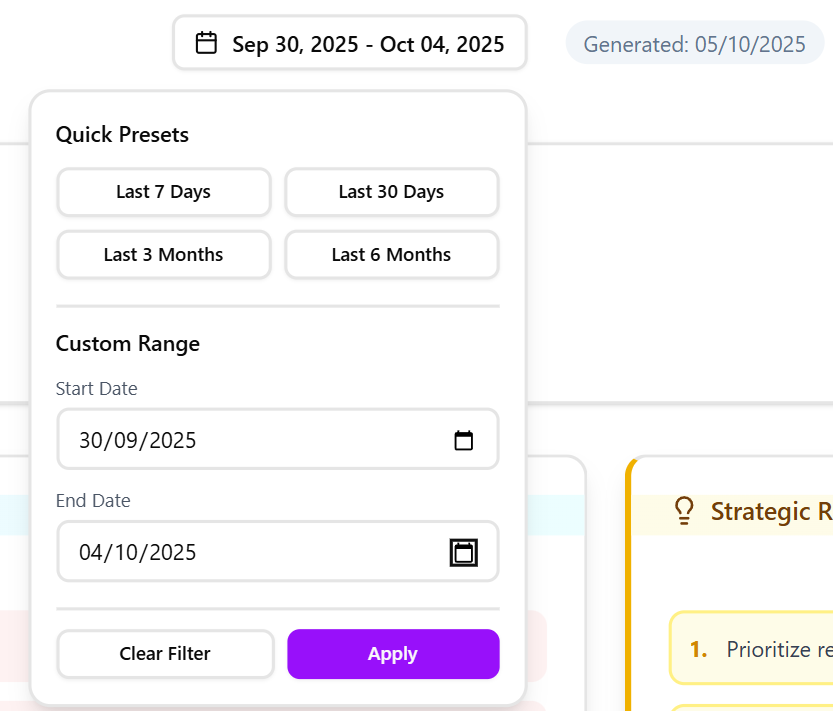
\includegraphics[width=0.7\linewidth]{img/chap_07/screenshot_date_filter..png}
    \caption{Date Range Filter with Quick Presets}
    \label{fig:date_filter}
\end{figure}

The date filter component (Figure 7.8) provides quick presets including Last 7 Days for recent activity, Last 30 Days for monthly trends, Last 3 Months for quarterly analysis, and Last 6 Months for long-term patterns. Custom selection allows precise start and end date specification using calendar picker with date validation. Real-time filtering applies selected range across all dashboard components updating charts, statistics, and tables automatically.

\subsection{PDF Export Progress Tracking}

Figure 7.9 displays the PDF export functionality with progress tracking interface.

\begin{figure}[H]
    \centering
    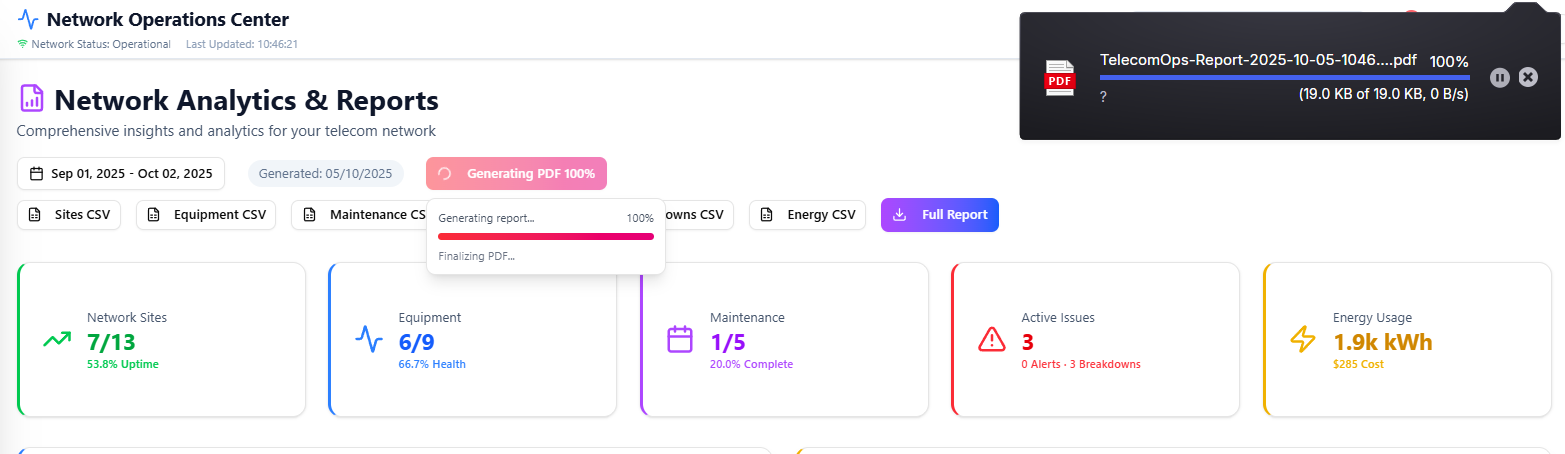
\includegraphics[width=1\linewidth]{img/chap_07/screenshot_pdf_export.png}
    \caption{PDF Export with Progress Tracking}
    \label{fig:pdf_export}
\end{figure}

The PDF export system (Figure 7.9) uses jsPDF for client-side generation with staged processing including preparation phase initializing document, summary phase adding executive overview, metrics phase formatting KPIs table, breakdowns phase adding detailed analysis, and finalization phase adding branding and page numbers. Progress tracking displays five distinct stages with visual progress bar showing 0-100% completion and status messages explaining current operation. This feedback prevents user confusion during generation providing clear indication of ongoing processing.

\subsection{Generated PDF Report Sample}

Figure 7.10 shows a sample of the generated PDF report with professional formatting.

\begin{figure}[H]
    \centering
    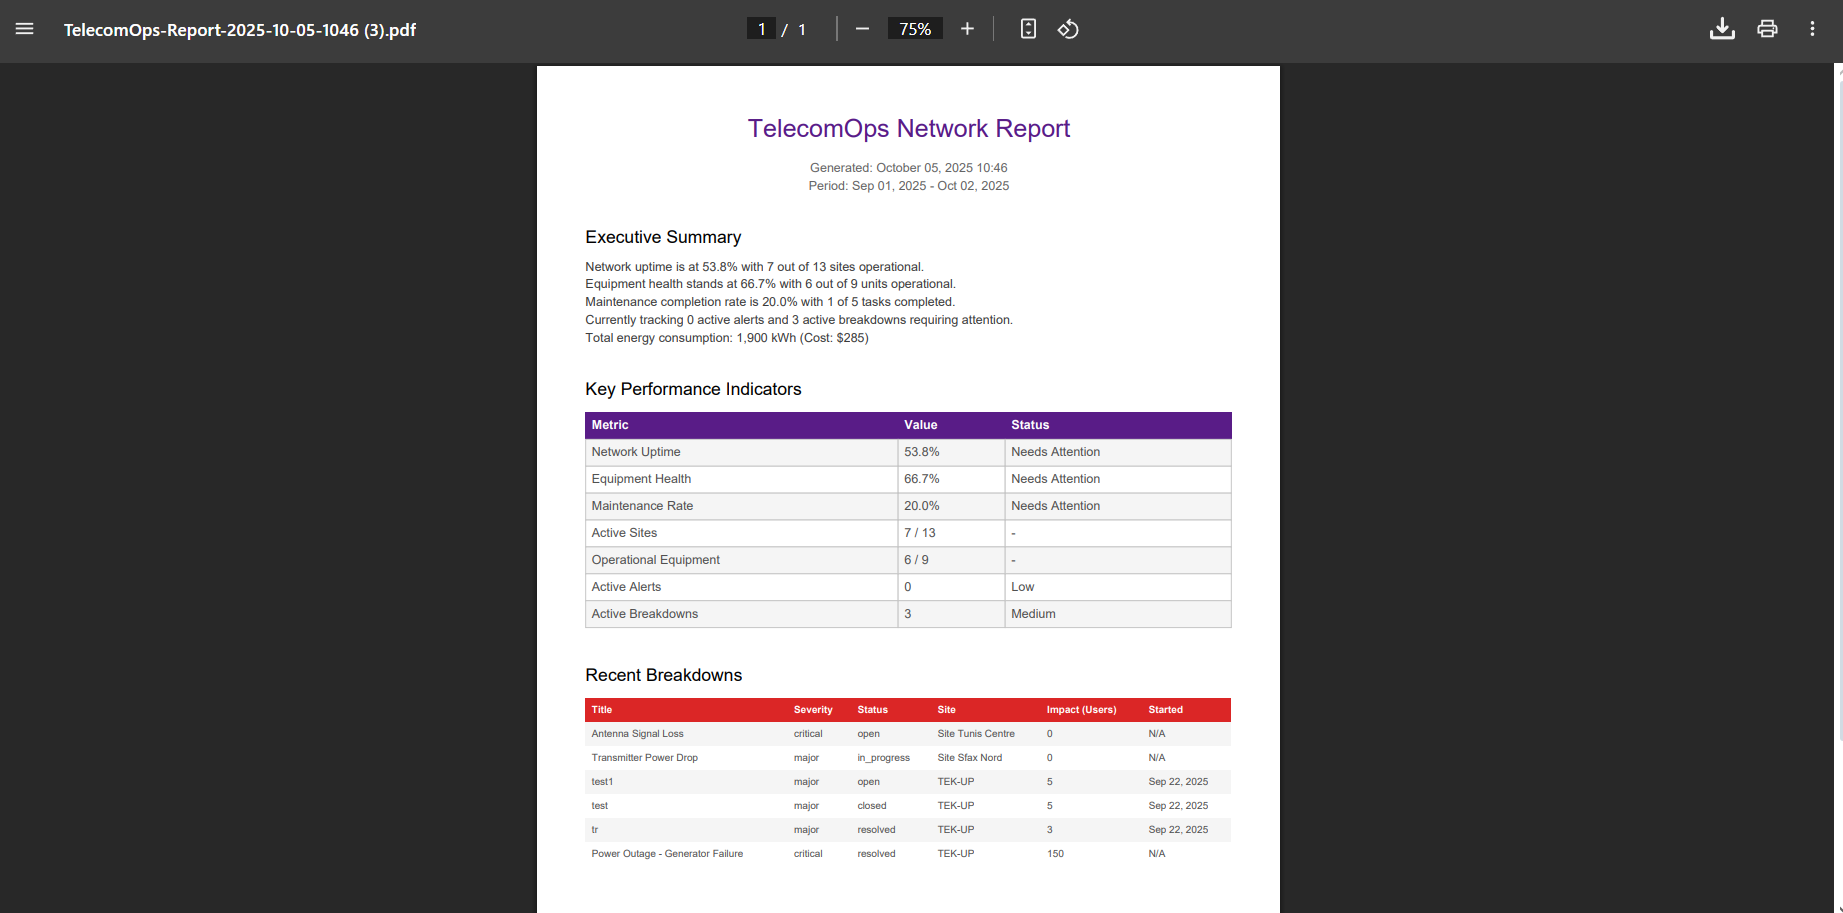
\includegraphics[width=0.9\linewidth]{img/chap_07/screenshot_pdf_sample.png}
    \caption{Generated PDF with Summary and Metrics}
    \label{fig:pdf_sample}
\end{figure}

The generated PDF (Figure 7.10) includes professional formatting with header displaying report title and timestamp, executive summary highlighting key findings, KPIs table showing critical metrics in structured format, and breakdown details with status and resolution information. Consistent branding throughout document with footer containing page numbers supports multi-page reports. The format enables distribution to stakeholders and archival for compliance requirements.

\section{Technical Challenges and Solutions}

Sprint 5 implementation encountered technical challenges requiring optimization and careful architecture decisions.

\subsection{Large Dataset Performance Optimization}

\textbf{Challenge:} Generating reports from extensive historical data spanning thousands of records required query optimization, memory management, and responsive user experience maintenance.

\textbf{Solution:} Database-level optimization implemented materialized views for pre-calculated metrics and compound indexes for faster joins across multiple tables. Application-level optimization uses incremental data loading fetching results in batches, lazy chart rendering loading visualizations on-demand, and virtual scrolling for large tables. For extremely large datasets exceeding browser capabilities, the system triggers background processing with email notification and secure download links ensuring user experience remains smooth.

\subsection{Client-Side PDF Generation Constraints}

\textbf{Challenge:} Browser-based PDF generation faced memory constraints limiting document size, table formatting complexity requiring proper sizing and wrapping, UTF-8 text encoding for multilingual support, and need for progress feedback during generation.

\textbf{Solution:} Implementation uses jsPDF with staged generation processing document in five distinct phases each updating progress indicator. Table formatting leverages autoTable plugin providing automatic column sizing, text wrapping, and page breaks. UTF-8 encoding configured properly supports Arabic, French, and English content. Memory-optimized batching processes large datasets in chunks preventing browser crashes while maintaining document quality.

\subsection{Real-Time Dashboard Updates}

\textbf{Challenge:} Maintaining dashboard accuracy with live data required efficient change detection, appropriate update frequency management, and proper handling of concurrent user sessions.

\textbf{Solution:} Hybrid update strategy combines Supabase real-time subscriptions for critical data changes (new alerts, equipment status) with intelligent polling for aggregated statistics updating every 30 seconds. React Query implements background refetching with stale-while-revalidate pattern and optimistic updates showing changes immediately. Components use React.memo hooks preventing unnecessary re-renders and batched state updates reducing performance impact.

\section{Testing and Validation}

Sprint 5 underwent comprehensive testing ensuring reliability and proper data aggregation.

\subsection{Functional Testing}

Report generation testing validated network summary reports aggregating site and equipment data, equipment status reports showing operational metrics, maintenance history reports from intervention data, and breakdown analysis reports with MTTR/MTBF calculations. Chart rendering confirmed correct visualization across various data distributions including empty states, single data points, and large datasets. Export functionality validated CSV format with proper encoding, JSON structure with metadata, and PDF generation with multi-page formatting. All export formats tested with special characters and large datasets.

\subsection{Integration Testing}

Data source integration verified correct aggregation from sites table (Sprint 1), equipment records (Sprint 2), interventions and breakdowns (Sprint 3), alerts (Sprint 4), and energy consumption (Sprint 4). Authorization testing confirmed role-based access with technicians viewing basic reports, managers accessing team analytics, engineers performing root cause analysis, and administrators generating executive reports. Export integration validated CSV compatibility with Excel and Google Sheets, JSON parsing in external tools, and PDF rendering across multiple PDF readers.

\subsection{Performance Testing}

Performance validation confirmed dashboard loading under 2 seconds with 1000+ records, chart rendering completing within 1 second for complex visualizations, report generation under 3 seconds for typical date ranges, CSV export processing 10,000 records in under 5 seconds, and PDF generation completing within 10 seconds for comprehensive reports. Memory profiling confirmed no leaks during repeated operations and efficient garbage collection.

\subsection{User Acceptance Testing}

Tunisia Telecom staff tested reporting capabilities in realistic scenarios. Management appreciated clear KPI presentation, automated metric calculation replacing manual compilation, and professional PDF reports for stakeholder distribution. Engineers valued breakdown analysis capabilities, maintenance trend visualization, and custom filtering for detailed investigation. Field supervisors confirmed mobile usability accessing reports from tablets during site visits. Overall feedback highlighted significant time savings and improved decision-making quality through accessible data insights.

\section{Sprint Review and Retrospective}

Sprint 5 review with stakeholders confirmed successful delivery of all committed user stories addressing US-012, US-013, and US-014 from Chapter 2's product backlog. Stakeholders particularly valued the comprehensive analytics dashboard, interactive visualizations, and professional PDF export. Management emphasized value from automated KPI calculation and trend analysis supporting strategic planning.

The sprint retrospective identified positive outcomes including successful data aggregation from all previous sprints, efficient query performance through materialized views, excellent user feedback on visualizations, and smooth PDF generation implementation. Technical achievements included sub-2-second dashboard performance and memory-efficient large dataset handling. Areas for improvement include additional chart types for specialized analysis, scheduled report generation for regular distribution, and enhanced mobile chart interactions.

\section{Conclusion}

Sprint 5 successfully delivered comprehensive reporting and analytics capabilities transforming operational data from Sprints 1-4 into actionable intelligence. The implementation addressed all committed user stories from Chapter 2's product backlog providing complete analytics dashboard, custom report generation, and multi-format export functionality.

The analytics dashboard provides unified operational visibility aggregating metrics from sites (Sprint 1), equipment (Sprint 2), maintenance activities (Sprint 3), and alerts and energy data (Sprint 4) through intuitive visualizations supporting both tactical operations and strategic planning. Interactive charting with drill-down capabilities enables trend identification and comparative analysis. Date range filtering with presets and custom selection provides flexible period analysis across all components.

Export functionality supporting CSV, JSON, and PDF enables external integration and stakeholder distribution. PDF generation with progress tracking delivers professional reports with consistent branding. Performance optimization through materialized views and intelligent caching ensures responsive experience with large datasets.

Technical achievements demonstrate production-ready reporting infrastructure with sub-2-second dashboard performance, efficient aggregation processing thousands of records, memory-optimized PDF generation, and hybrid update strategy balancing real-time accuracy with performance. Quality metrics exceeded Chapter 2's NFR-001 requirements with comprehensive stakeholder validation.

The reporting system establishes foundation for advanced analytics including predictive maintenance forecasting future failures, anomaly detection identifying unusual patterns, automated insight generation highlighting critical trends, and machine learning integration supporting optimization recommendations. Sprint 5 completes the core TelecomOps platform delivering end-to-end network management capabilities from site tracking through advanced analytics supporting Tunisia Telecom's operational excellence objectives.

The next chapter presents the General Conclusion, synthesizing achievements across all five sprints, evaluating project outcomes against initial objectives from Chapter 1, and discussing future enhancements and strategic recommendations for continued platform evolution.